%
% File acl2013.tex
%
% Contact  navigli@di.uniroma1.it
%%
%% Based on the style files for ACL-2012, which were, in turn,
%% based on the style files for ACL-2011, which were, in turn, 
%% based on the style files for ACL-2010, which were, in turn, 
%% based on the style files for ACL-IJCNLP-2009, which were, in turn,
%% based on the style files for EACL-2009 and IJCNLP-2008...

%% Based on the style files for EACL 2006 by 
%%e.agirre@ehu.es or Sergi.Balari@uab.es
%% and that of ACL 08 by Joakim Nivre and Noah Smith

\documentclass[11pt]{article}
\usepackage{acl2013}
\usepackage{times}
\usepackage{url}
\usepackage{latexsym}

\usepackage{graphicx}
%\setlength\titlebox{6.5cm}    % You can expand the title box if you
% really have to

\title{CoolName2k: Longitudinal Web Sampling for Fun and Profit}

\author{Stephen Wattam \\\And
  Paul Rayson\\\And
  Damon Berridge\\\AND
  Lancaster University\\
  {\tt f.lastname@lancs.ac.uk}\\
}


\date{}

\begin{document}
\maketitle

\section{Sampling}

Many sampling efforts for linguistic data on the web are heavily focused on producing results comparable to conventional corpora.  These typically take two forms: those based on URI lists (typically derived from search engine data, as in~\cite{sharoff2006creating}), and those formed through crawling.

Though initial efforts in WaC first focused on the former, in part due to concerns over the balance of samples returned, many projects are now focused on constructing supercorpora, which may themselves be searched with greater precision than the 'raw' web, in line with Kilgarriff's vision of linguistic search engines~\cite{kilgarriff2003linguistic}.  This has led to the proliferation of crawlers such as those mentioned in~\cite{schafer8building} and~\cite{renouf2003webcorp}.

% diachronic work with webcorp.
% \cite{kehoe2006diachronic}
% \cite{kehoe2009weaving}

This approach, with its base in a continually-growing supercorpus, parallels the strategy of a monitor corpus~\cite{sinclair1982monitor}, and is applicable to a linguistic inquiry concerned with diachronic properties~\cite{kehoe2006diachronic}.  Indeed, we could conclude that the web is mature enough to require date-based lookup when retrieving articles, and such tools are increasingly being included in consumer search engines such as Google.

This repeated sampling approach tells us about the state of language change online in a manner that is immediately comparable to other diachronic corpora, however, it omits subtler technical aspects that govern consumption of data online, most notably the URI of the data, and variation in where this points over time.  Low publishing costs online, paired with increasing corporate oversight and reputation management, leads to a situation where this content is being updated frequently, often without end users even noticing.

This URI-oriented change has been studied from a technical perspective by those interested in managing and maintaining network infrastructure, and optimising the maintenance of search engine databases~\cite{koehler2004longitudinal}.  The needs of these parties are quite aside from those of corpus researchers, however, since they focus around a best-effort database of information, rather than a dependable sample (which must have known margins for error).
% 
% \begin{itemize}
%     \item \textsl{Incremental sampling}---Search engine databases and digital archives are persistent, and may be incrementally updated in a continuous manner whilst still being useful;
%     \item \textsl{Lack of comparability}---A cross-sectional sample of search databses yields documents sampled at various times, with a possible age variation as modelled by the specific type of web page.  This is evidenced well by the relative likelihood of receiving a broken link when searching for current events \textsl{vs.} older scientific articles.
%     \item \textsl{Information-seeking behaviour}---Search engine literature indicates [CITE] that information, when lost from one location, is often available at many others.  This same process is unlikely to be followed, however, if a resource has simply changed, or if a user relies on a small set of web pages as an information resource (such as news sources).
%     \item \textsl{Deliberate `usefulness bias'}---Sources deemed to be pertinent to a search engine's clientelle are sampled more frequently, and thoroughly.  This results in persistence-of-value surrounding high-profile domain names and companies, which dominate the zipfian distribution of web results.
% \end{itemize}
% 


We present here a tool for this form of longitudinal sampling, designed to maximise the comparability of documents downloaded in each sample in terms of their URI rather than content.  To accomplish this, we use a batch-mode sampling strategy, as illustrated in Figure~\ref{fig:sampling}, to get full coverage over a list of URIs, at the expense of sampling new content.

\begin{figure}[h]
\centering
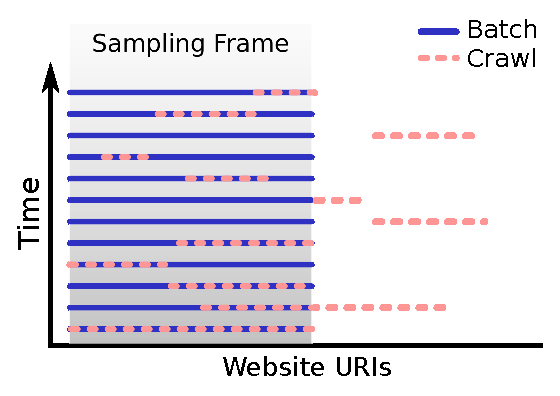
\includegraphics[width=0.4\textwidth]{images/samples.eps}
\caption{URI coverage for batch and crawl.}
\label{fig:sampling}
\end{figure}

\section{Aims}
The tool is designed to construct longitudinal samples from URI lists, using only commodity hardware.  It is designed with `full storage' in mind, that is, recording everything about each HTTP session in such a way that it may later be exported and accessed in a parsimonious manner.

\section{Architecture}

\begin{figure}[h]
\centering
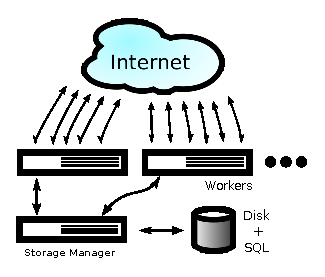
\includegraphics[width=0.4\textwidth]{images/arch.eps}
\caption{System Architecture}
\label{fig:arch}
\end{figure}
In order to maximise the simultaneity of a given sample, a parallel, distributed architecture was selected (Figure~\ref{fig:arch}).  This also yields technical benefits of throughput (especially where the internet connection is a bottleneck), and the ability to differentiate between websites that are blocked for a given area of the internet and those that are offline `proper'.

Data storage in the system is split between metadata, stored in an SQLite database, and website sample data itself, which is stored as raw HTTP response data in a versioned structure, compressed using hard links\footnote{Linked in a similar manner to \texttt{rsync}'s \texttt{-H} option.}.  The storage format is optimised for large samples, and is nested in order to avoid common filesystem limits.

The download process itself is managed by a central server, which co-ordinates storage and metadata access in order to provide atomicity and recording of sample data.  This central server distributes batch jobs, according to policies governing reliability and throughput, to worker servers, which compete for the opportunity to download websites.

Workers imitate, as far as possible, the behaviour of real users.  They retain cookies and present typical user-agent and referrer strings in their request headers.

\section{Performance}
In order to obtain the most simultaneous samples, the system was designed to maximise the parallel number of connections on each client.  This eventually led to exceeding the limits of the underlying operating system, which in our tests showed a practical maximum of 120 simultaneous downloads\footnote{Using the Linux 2.8 kernel}.

In practice, throughput is defined both by the external servers and this parallelism limit---reducing timeouts for failed DNS and HTTP connections leads to significant improvements later on in a sample where many hosts have fallen offline.  With low failure rates, the system is capable of downloading millions of pages in a 24-hour period.

As with many downloaders, it is possible to exceed polite limits of server usage with an internet connection of even modest throughput.
% The original uses for the tool required sampling once or twice per server, meaning this was not a significant problem, however, those wishing to download websites will find themselves dealing with significant ethical concerns.

\section{Applications}

Corpora built using this strategy offer insights into the properties of language as it is used and maintained on a daily basis, yielding particular value to epistemic problems regarding web sampling:

\begin{itemize}
    \item The proportions and areas of web pages that typically change as boilerplate and templating systems;
    \item The impact of social feedback and user generated content on page content;
    \item How censorship, redaction and revision affect website contents;
    \item Website resource persistence relative to content (link rot/document attrition).
\end{itemize}



\bibliographystyle{acl}
% you bib file should really go here 
\bibliography{downloadtools}

\end{document}
